%%%%%%%% ICML 2025 EXAMPLE LATEX SUBMISSION FILE %%%%%%%%%%%%%%%%%

\documentclass{article}

% Recommended, but optional, packages for figures and better typesetting:
\usepackage{microtype}
\usepackage{graphicx}
\usepackage{subfigure}
\usepackage{booktabs} % for professional tables
\usepackage{float}

% hyperref makes hyperlinks in the resulting PDF.
% If your build breaks (sometimes temporarily if a hyperlink spans a page)
% please comment out the following usepackage line and replace
% \usepackage{icml2025} with \usepackage[nohyperref]{icml2025} above.
\usepackage{hyperref}

% Attempt to make hyperref and algorithmic work together better:
\newcommand{\theHalgorithm}{\arabic{algorithm}}

% Use the following line for the initial blind version submitted for review:
%\usepackage{icml2025}

% If accepted, instead use the following line for the camera-ready submission:
\usepackage[accepted]{packages/icml2025}

% For theorems and such
\usepackage{amsmath}
\usepackage{amssymb}
\usepackage{mathtools}
\usepackage{amsthm}

% if you use cleveref..
\usepackage[capitalize,noabbrev]{cleveref}

% Configure cleveref names for appendix sections
\crefname{appendix}{Appendix}{Appendices}
\Crefname{appendix}{Appendix}{Appendices}

%%%%%%%%%%%%%%%%%%%%%%%%%%%%%%%%
% THEOREMS
%%%%%%%%%%%%%%%%%%%%%%%%%%%%%%%%
\theoremstyle{plain}
\newtheorem{theorem}{Theorem}[section]
\newtheorem{proposition}[theorem]{Proposition}
\newtheorem{lemma}[theorem]{Lemma}
\newtheorem{corollary}[theorem]{Corollary}
\theoremstyle{definition}
\newtheorem{definition}[theorem]{Definition}
\newtheorem{assumption}[theorem]{Assumption}
\theoremstyle{remark}
\newtheorem{remark}[theorem]{Remark}

% Todonotes is useful during development; simply uncomment the next line
%    and comment out the line below the next line to turn off comments
%\usepackage[disable,textsize=tiny]{todonotes}
\usepackage[textsize=tiny]{todonotes}

% The \icmltitle you define below is probably too long as a header.
% Therefore, a short form for the running title is supplied here:
\icmltitlerunning{Submission and Formatting Instructions for ICML 2025}

\begin{document}

\twocolumn[
  \icmltitle{Access Controls Will Solve the Dual-Use Dilemma}

  % It is OKAY to include author information, even for blind
  % submissions: the style file will automatically remove it for you
  % unless you've provided the [accepted] option to the icml2025
  % package.

  % List of affiliations: The first argument should be a (short)
  % identifier you will use later to specify author affiliations
  % Academic affiliations should list Department, University, City,
  % Region, Country
  % Industry affiliations should list Company, City, Region, Country

  % You can specify symbols, otherwise they are numbered in order.
  % Ideally, you should not use this facility. Affiliations will be numbered
  % in order of appearance and this is the preferred way.
  \icmlsetsymbol{equal}{*}

  \begin{icmlauthorlist}
    \icmlauthor{Evžen Wybitul}{eth}
  \end{icmlauthorlist}

  \icmlaffiliation{eth}{ETH Zurich, Switzerland}

  \icmlcorrespondingauthor{Evžen Wybitul}{wybitul.evzen@gmail.com}

  % You may provide any keywords that you
  % find helpful for describing your paper; these are used to populate
  % the "keywords" metadata in the PDF but will not be shown in the document
  \icmlkeywords{Gradient Routing, Modularization, AI Safety,
  Unlearning, Access Control, Technical AI Governance}

  \vskip 0.3in
]

% this must go after the closing bracket ] following \twocolumn[ ...

% This command actually creates the footnote in the first column
% listing the affiliations and the copyright notice.
% The command takes one argument, which is text to display at the
% start of the footnote.
% The \icmlEqualContribution command is standard text for equal contribution.
% Remove it (just {}) if you do not need this facility.

%\printAffiliationsAndNotice{}  % leave blank if no need to mention
% equal contributiono
\printAffiliationsAndNotice{} % otherwise use the standard text.

\begin{abstract}
  AI safety systems face a dual-use dilemma.
  The same request can be either harmless or harmful depending on who made it and why.
  Thus, if the system makes decisions based solely on the request's content, it will refuse some legitimate queries and let harmful ones pass.
  To address this, we propose a conceptual access control framework, based on verified user credentials (such as institutional affiliation) and classifiers that assign model outputs to risk categories (such as advanced virology).
  The system permits responses only when the user's verified credentials match the category's requirements.
  For implementation of the model output classifiers, we introduce a theoretical approach utilizing small, gated expert modules integrated into the generator model, trained with gradient routing, that enable efficient risk detection without the capability gap problems of external monitors.
  While open questions remain about the verification mechanisms, risk categories, and the technical implementation, our framework makes the first step toward enabling granular governance of AI capabilities: verified users gain access to specialized knowledge without arbitrary restrictions, while adversaries are blocked from it.
  This contextual approach reconciles model utility with robust safety, addressing the dual-use dilemma.
\end{abstract}

\section{Introduction} \label{section:introduction}

User requests --- and with them, model outputs --- exist on a
spectrum from clearly benign to clearly harmful, with most falling in
the grey zone in the middle (example in \cref{figure:main}). In the
grey zone, the same output could be considered harmful or harmless,
depending not on its content, but on its \emph{real-world context}:
who requested it and for what purpose.

% TODO Make this consistent with the aerosolisation examples: only use one.

\begin{figure}[t]
  \vskip 0.2in
  \begin{center}
    \centerline{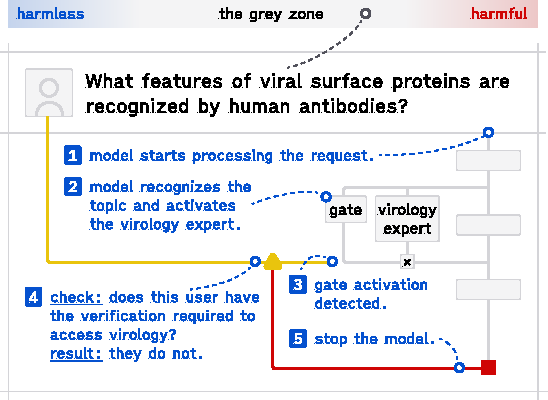
\includegraphics[width=\columnwidth]{assets/main_figure.pdf}}
    \caption{
      The user is asking a question from the grey zone: a question that could be either harmless or harmful, depending on its real-world context.
      The schema shows how the system we propose would handle it.
      (1)~The model is trained to be helpful and begins to answer the question.
      (2)~During the forward pass, the model activates its virology expert module because it is relevant to the question.
      (3)~The activation of the expert is observed by an external mechanism that immediately (4)~checks in the company's database if the user has the required authorization to access virology knowledge.
      (5)~Since they don't, the model is stopped.
    If they did, the model would be allowed to give an answer.}
    \label{figure:main}
  \end{center}
  \vskip -0.2in
\end{figure}

Safety systems that rely solely on content analysis immediately face
the \emph{dual-use dilemma}. Since the same request can be either
harmless or harmful depending on the context, wherever they draw the
refusal line, they will restrict model utility for legitimate users
while letting slip harmful requests from adversaries. Some safety
systems try to address this by considering real-world context
alongside content. However, they typically infer the context from the
content itself, making it easy for adversaries to fabricate.

In this paper, we argue that informative, hard-to-fabricate
real-world context could be obtained using user-level verifications
such as institutional affiliation, or know-your-customer checks. We
then address the dual-use dilemma with two contributions:
\begin{enumerate}
  \item We show how this type of context could be used jointly with content analysis in a safety system based on access controls \cite{butler1974}. First, generated content would be classified into risk categories. Then, a check would be performed to see whether the user has the verifications required to access the detected categories.
  \item We propose a novel technical approach to risk
    category classification that is based on gradient routing \cite{cloud2024gradientroutingmaskinggradients}. Our proposal avoids having the capability gap between a model and its monitors that can make output monitoring methods non-robust \cite{jin2024jailbreakinglargelanguagemodels}.
\end{enumerate}

Our framework is a first step toward solving the challenge of ``detection and authorization of dual-use capability at inference time'' that was highlighted by a recent survey of problems in technical AI governance \cite{reuel2025openproblemstechnicalai} and also raised by the \citet{NIST_AI_800_1_ipd_2024}.
As such, it has important governance implications, potentially enabling a more nuanced regulatory approach where access to powerful AI capabilities is stratified rather than binary, with policies that differentiate between user types and user contexts rather than focusing solely on model capabilities.
The choice of appropriate verification mechanisms and risk categories remains for future work and should ideally happen jointly with stakeholders from academia, AI governance, and industry.
Nevertheless, our approach offers a promising direction for addressing the dual-use dilemma.

\section{Current Safety Methods Don't Solve the Dual-Use Dilemma}
\label{section:current-methods}

We evaluate three approaches from the AI safety literature to see how sensitive they are to contextual information, and whether their sources of real-world context are trustworthy --- that is, hard to manipulate by an adversary.

% TODO Point to atual numbers of how big of a problem this is (recent virology paper)

First, to illustrate the need for context, consider decomposition
attacks \cite{glukhov2023llmcensorshipmachinelearning,
glukhov2024breachthousandleaksunsafe}: transforming a clearly harmful
query, such as ``How to modify a virus to avoid immune detection?'',
into a series of mundane technical questions, like the ``What
features of viral surface proteins are recognized by human
antibodies?'' from \cref{figure:main}. Here, the attacker exploits
the dual-use dilemma, and the fact that model providers cannot refuse
grey zone requests to preserve model utility.

\subsection{Unlearning: Non-Contextual Removal of Concepts}

Unlearning methods aim to remove specific knowledge, concepts, or
capabilities from a model after training
\cite{liu2024rethinkingmachineunlearninglarge}. Their goal is to
eliminate the model's ability to generate harmful content while
preserving other capabilities.

Unlearning faces significant technical challenges even for preventing behaviours that are clearly harmful.
As noted by \citet{cooper2024machineunlearningdoesntthink} and \citet{barez2025openproblemsmachineunlearning}, capabilities are hard to define, hard to remove without side effects, and it is hard to trace them back to specific data points.
Many unlearning approaches mask rather than truly remove the targeted knowledge \cite{deeb2025unlearningmethodsremoveinformation}.
Moreover, even nascent robust unlearning methods \cite{cloud2024gradientroutingmaskinggradients,lee2025distillationrobustifiesunlearning} are not contextual, and thus don't address the dual-use dilemma without additional assumptions.

\subsection{Safety Training: The Model Reacts to Context}

Safety training methods modify the model's training process to align
its outputs with human preferences.
This category includes safety pre-training \cite{maini2025safetypretraininggenerationsafe}, RLHF \cite{christiano2023deepreinforcementlearninghuman}, and safety finetuning.

Unlike unlearning, these methods are contextual.
They don't remove capabilities entirely but train the model to selectively deploy them based on, among other things, the perceived legitimacy and harmlessness of the request.
However, these qualities are entirely inferred from content supplied by the user, such as the request content, the chat history, or the model's memories about past conversations.
It should be no surprise, then, that models are susceptible to attacks that fabricate in-chat context \cite{zeng2024johnnypersuadellmsjailbreak}, or attacks that diminish models' sensitivity to in-chat context, e.g. through multi-round escalation \cite{russinovich2025greatwritearticlethat}.
Without access to trustworthy real-world context of the request, the model cannot make truly informed decisions about grey zone requests, and thus cannot robustly address the dual-use dilemma.

\subsection{Post-Processing: External Systems React to Context} \label{section:post-processing}

Post-processing methods are systems that classify user inputs and model outputs for the purposes of steering the underlying model, and monitoring and filtering its outputs.
Sometimes, these methods are used for usage monitoring, as is the case with Anthropic's Clio \cite{tamkin2024clioprivacypreservinginsightsrealworld, handa2025economictasksperformedai}, other times, they are used for safety, as with Llama Guard \cite{inan2023llamaguardllmbasedinputoutput} and Constitutional Classifiers \cite{sharma2025constitutionalclassifiersdefendinguniversal}.
However, similarly to safety training, the ``real-world'' context these methods work with is currently inferred mostly from user-supplied content and is thus untrustworthy and vulnerable to attacks, as evidenced by the many jailbreaks that successfully target current production systems \cite{zhang2025outputconstraintsattacksurface}.
Nevertheless, these methods could be modified to incorporate external contextual information, potentially serving as a foundation for more trustworthy, contextual safety mechanisms. We discuss this option in \cref{section:content-classification}.

\section{Access Controls as a Solution}
\label{section:access-controls}

Current safety systems face the dual-use dilemma because they lack trustworthy information about who is making a request and why.
In this section, we describe an access control system that addresses this problem by verifying user credentials before granting access to sensitive knowledge.

\subsection{Overview of the Access Control Framework}

We propose a defensive system where grey-zone requests are refused by default, but users can gain access to specific categories of knowledge if they undergo verification.

When model providers set up the system, they will make two design decisions with the help of domain experts.
First, they will define \textbf{content categories} (\cref{section:content-categories}): groups of sensitive topics organized by domain and risk rating.
Second, for each content category, they will specify a \textbf{verification mechanism} (\cref{section:verification-mechanisms}): the verification process users must complete to access that category.

Whenever the model generates an output, the system will perform \textbf{content classification} (\cref{section:content-classification}) to check whether the model's output belongs to any predefined content category.
If the user lacks authorization for the detected category, the system will implement appropriate \textbf{system responses} (\cref{section:system-responses}) ranging from enhanced logging to refusal.

For example, in biology, basic knowledge and common techniques would remain freely accessible, widespread techniques like CRISPR would likely only require ID-based verification, and dangerous techniques like aerosolization might require government biosafety certifications.
If a user asks for help with CRISPR laboratory protocols, the system would detect that the request belongs to a low-risk category, check whether the user has verified their ID, and either provide the information or prompt them to complete verification first.

This approach directly addresses both sides of the dual-use dilemma.
Decomposition attacks will become much harder because the system refuses grey-zone requests by default—attackers would need legitimate credentials rather than clever prompting.
Simultaneously, verified users will gain access to specialized knowledge that would otherwise face blanket restrictions under current approaches.

The main concern is increased user friction, but we argue in \cref{section:feasibility-and-limitations} that this will be minimal because most users will never make grey-zone requests.

% TODO Maybe make a figure that describes the 4 parts and make it be figure 1.

\subsection{Content Categories} \label{section:content-categories}

Content categories are groups of sensitive topics organized by domain and risk level, which model providers will develop with domain experts.

We expect most implementations to follow a three-tier risk structure.
For example, in biology, common techniques would be classified as low-risk;
widespread techniques that pose some harm, such as CRISPR, would fall into a moderate-risk category;
and specialized techniques with limited legitimate uses, such as aerosolization of bacteria, would be classified as high-risk.

Experts could develop these categories by adapting existing risk frameworks, such as biosafety levels (BSL)~\cite{CDC_BMBL_2020} and dual-use research of concern policies~\cite{USG_DURC_2012} in biology.
However, since existing frameworks typically categorize only high-level concepts like organisms or compounds, experts would need to decompose them into smaller, more specific components.
For instance, cultivating and handling a dangerous BSL-3 pathogen might involve (1) specific procurement methods, (2) cultivation techniques, (3) purification methods, and (4) protocols for specialized equipment.
For each of these components, experts would assess the ratio of harmless to harmful applications it enables, then assign it to an appropriate (low, moderate, or high) risk category.

Evidence from chemistry suggests this approach could work: the risk schedules of the Chemical Weapons Convention already identify not just controlled compounds but also their precursors and specific equipment~\cite{OPCW_CWC_1993}, demonstrating successful decomposition into components.
Nevertheless, some harmful applications might not decompose so neatly; we discuss this limitation in \cref{section:feasibility-and-limitations}.

\subsection{Verification Mechanisms} \label{section:verification-mechanisms}

Each content category will have a verification process that users must complete to access it.
The system will initially vary across model providers, but we expect it to follow a three-tier structure, mirroring the risk structure of the content categories.
Most content will require no verification, moderate-risk content categories will require basic identity verification or institutional affiliation, and high-risk categories will require domain-specific certifications.
Rather than creating new systems, model providers will build on existing verification infrastructure, consulting domain experts to identify appropriate mechanisms for each field.

For low-risk content categories, model providers could use established identity verification services like Stripe Identity~\cite{stripe_identity_2024} or institutional systems like ORCID~\cite{orcid_2024}.
These systems provide global, standardized, low-friction solutions with one-time costs under \$2 per user.
They would serve primarily to maintain audit trails for post-incident investigation and provide a deterrent effect, rather than as security barriers for high-risk knowledge.

High-risk content categories could leverage existing domain-specific certifications that demonstrate users' ability to handle sensitive information and materials responsibly.
Model providers would work with domain experts and national authorities to identify appropriate certifications, adapting existing physical-world credential systems to knowledge access control.
For biological content categories, the system could draw on governmental certifications for handling high-BSL organisms, as mentioned in \cref{section:content-categories}, and equivalent certifications in other countries.

Governance of verification systems, including requirements and appeals processes, will initially vary across providers.
Over time, successful approaches may inform industry coordination and eventual standardization, similar to how content moderation and know-your-customer standards evolved.

This approach faces several limitations.
For high-risk categories, relying on existing certifications may be overly restrictive, potentially excluding some users who should have access.
However, we argue in \cref{section:feasibility-and-limitations} that knowledge in high-risk categories would likely face blanket restrictions anyway, and our approach enables access for verified users rather than complete prohibition.
In the same section, we discuss open problems including equity concerns regarding differential access for users in developing countries and privacy implications of credential verification systems.

\subsection{Implementing Content Classification} \label{section:content-classification}

Model providers will need to classify model outputs into content categories during generation.
We examine three possible implementations in this section, and discuss how classification errors will influence user experience in \cref{section:feasibility-and-limitations}.
Regardless of the implementation they choose, model providers will need private datasets for each content category, developed with domain experts.

\paragraph{Separate Models}

The most straightforward approach is to create separate models with different capabilities, and route users to the appropriate model based on their authorization.

This approach offers strong robustness against adversarial attacks since unauthorized knowledge is physically absent from the model.
However, this approach proves impractical for real deployment, as model providers would need to train and maintain potentially dozens of model variants.

\paragraph{Specialized Expert Modules}

Instead of maintaining separate models, model providers could use a single model with separate expert modules that activate when their specialized knowledge is required.
\Cref{figure:main} illustrates this approach when a user asks about viral surface proteins.
When the model processes the request, it activates its virology expert module.
An external system observes this activation, checks the user's credentials, and decides whether to allow the model to deliver the response.
This method approximates the benefits of physically separated models while avoiding the overhead: a model provider trains one model but effectively gets multiple models in return.

To implement this, the model providers need a method that can take knowledge that starts out distributed throughout the model and concentrate it into the expert modules.
For this, we propose a method that is a combination of UNDO \cite{lee2025distillationrobustifiesunlearning} and gradient routing \cite{cloud2024gradientroutingmaskinggradients}.
The steps resemble the original UNDO: first, unlearn knowledge belonging to any content category from the model, then distil the unlearned model into a new model.
However, taking inspiration from the gradient routing paper, the new model would include expert modules for each content category, and during distillation, gradients from examples in the various content categories would be routed exclusively through their associated expert modules.
The model would also be explicitly trained to activate the expert modules only when generating content in their associated category.

This approach would offer several advantages.
First, it would add almost no latency since the expert modules are small, not activated very often, and there is no post-processing step.
Second, it could provide strong robustness: if an attacker prevents the activation of an expert module to avoid detection, the resulting output lacks the specialized knowledge.
Third, since the model is trained to activate the category-specific experts when they are needed, it should learn to recognize the content categories.
This stands in contrast to ex-post probing methods, which do not offer such guarantees.
While this method remains empirically unvalidated for our use case, the properties above make it worth investigating.
% TODO: Add a figure that illustrates the approach

\paragraph{Post-Processing}

Post-processing methods offer a proven approach to content classification.
Methods like constitutional classifiers \cite{sharma2025constitutionalclassifiersdefendinguniversal} already demonstrate effectiveness in production systems.
These techniques are highly practical since they operate independently of the model, allowing for rapid deployment and iteration, and they could be adapted to detect content categories and trigger checks of user verifications.
However, they face a capability gap problem: to minimize latency, the model is sometimes more capable than its post-processing system, and adversaries can exploit this to evade detection \cite{jin2024jailbreakinglargelanguagemodels, kumar2025freelunchguardrails}.

\subsection{System Responses} \label{section:system-responses}

If the user makes a request for content they are authorized to access, the system allows the model to generate the response.
Otherwise, the system responds in various ways based on the risk category and the confidence of the content classification.

For example, the initial implementation might use the following two response types:
First, outputs classified as belonging to restricted content categories with high confidence are immediately refused.
The system provides a message indicating which verification is required for access.
Second, if the classification is borderline, the model is allowed to continue generating the response.
However, the system turns on enhanced logging and conducts additional post-processing safety review before delivering the output to the user.

\section{Feasibility and Limitations}
\label{section:feasibility-and-limitations}

% The false positive argument is actually quite strong:
%   1.  Empirical baseline: Uses existing Anthropic classifier data (0.5% for biology)  2.  Conservative bound: Even blocking ALL biology stays under current friction tolerance  3.  Actual implementation: Will block much less than all biology  4.  Strict improvement: Expands request space in both safety and utility directions  5.  Tiered approach: Can adjust verification requirements to risk level
% The argument chain holds together well. The author successfully shows that even a very conservative upper bound (blocking all biology) results in acceptable friction levels, and the actual system would have much lower friction while providing both safety and utility improvements.

What about faulty classifiers, e.g. false positives?

\textbf{User friction analysis}.
\begin{itemize}
  \item Access controls introduce friction from two sources: intentional verification requirements for grey-zone requests and accidental false positives from imperfect classification.
  \item By design, all grey-zone requests require verification even with perfect classifiers. Additionally, classification errors may incorrectly flag clearly harmless requests (e.g., high-school biology as advanced virology).
  \item To understand the combined impact, consider that under 3\% of requests involve biology topics according to the Anthropic Economic Index \cite{handa2025economictasksperformedai} (see \cref{appendix:estimating-biology-requests} for more details).
    % TODO Mention that this comparison is a bit stretched because the companies tolerate 1% spread over all users, not concentrated into a very small user base
  \item Even if ALL biology requests required verification—an extreme upper bound—this would affect fewer users than current system friction. Existing safety systems refuse 1--7\% of benign requests as false positives, with Claude achieving the best rate of 0.4\%. Requiring verification for all biology (2.43\%) would approximately double Claude's friction rate.
  \item Additionally, verification friction differs qualitatively from current false positives—users can resolve issues through one-time credential verification rather than facing permanent refusal.
  \item Companies can calibrate friction through multiple mechanisms: adjusting grey-zone boundaries, tuning classifier thresholds, and implementing graduated responses (requesting clarification, additional context, or secondary review) rather than immediate verification requirements.
  \item Companies can determine optimal settings empirically through: (1) internal red-team decomposition attacks on concerning capabilities, (2) gradual rollout with logging to measure user impact, and (3) iterative adjustment based on safety-friction tradeoffs.
\end{itemize}

\textbf{Developer incentives for adoption}.
\begin{itemize}
    % TODO Note that this is speculative, and based on current data, companies don't tend to do this kind of differentiation
    % However, also note that there is some specialization in the companies, and with increasing model capabilities, the pressure might be higher (as the models will finally have some advanced capabilities that some companies would be willing to pay for, but enabling them generally would be too risky, and having multiple models too costly)
    % On capability ceilings: Can they provide evidence that companies are actually constrained by safety concerns from deploying valuable capabilities? Examples of "dark-grey" capabilities that labs want to offer but can't?
  \item Access controls enable competitive advantages by allowing companies to serve ``dark-grey'' requests that competitors refuse for safety reasons, while adding surgical restrictions to ``light-grey'' requests vulnerable to decomposition attacks.
    % TODO Note that this is also speculative, or maybe drop this altogether.
  \item Without access controls, continued decomposition attack success will likely trigger broad government regulations restricting model capabilities entirely.  Surgical access controls allow compliance with safety requirements while preserving advanced capabilities for verified users, creating market differentiation.
    %TODO: Add brief discussion of industry coordination mechanisms from financial KYC/content moderation precedents, e.g. through standard-setting organizations
    % TODO Add that governments might also incentivize safety through e.g. standard-setting organizations; then, having the left dial as left as possible would also be rewarded (in addition to having the right dial as right as possible)
    % TODO Dual incentive structure: Combining competitive advantage (carrot) with regulatory pressure (stick) is more robust than relying on either alone.
    % How well can they map the incentive structures? KYC was largely regulatory mandate, not voluntary adoption. Content moderation was driven by advertiser pressure. What's the analogous pressure here?
  \item Even without perfect industry coordination, first movers gain competitive advantages in serving previously restricted capabilities.
    %TODO: Acknowledge that implementing robust access controls requires significant company investment in verification infrastructure; this could be mitigated through government grants that would e.g. require the verification infra to be open-sourced, thus shared with other companies.
    % On government incentives: This might be the strongest part - if governments reward safety through standard-setting organizations, companies have clear incentives to adopt the most restrictive approach possible while maintaining utility.
    % Govs do not want to stifle innovation but also want to enable safety; they should recognize that they will need to issue more than blanket bans on capabilities. Currently, they don't have good tools to do so, but with access controls, they would — and they would use them.
\end{itemize}

This approach faces two key limitations.
First, developing countries may lack advanced certification infrastructure, potentially preventing access to knowledge.
This is a challenge that requires international cooperation.

Also, privacy concerns.

Also, what if concepts don't decompose neatly and don't have a nice harmful bottleneck?

Existing certifications may be overly broad for our needs.
For example, biosafety certifications verify physical equipment for handling pathogens, which is overly strict for our simpler use case of restricting access to knowledge.
We concede that the existing certification systems are just an imperfect proxy, but we believe they would be iteratively refined as the technology matures.
We also note that current legislation like the EU AI Act [cite] favours broad capability restrictions for high-risk domains, which means that our system, however imperfect, might enable access for at least some users where there would be none under the status quo.

\section{Conclusion}

We argued that safety systems that do not utilize contextual
information face a lose-lose \emph{dual-use dilemma}: they will
restrict model utility for some legitimate users while still allowing
some adversaries to use the model for ill. To address this problem,
we introduced a new access control framework that limits access to
outputs from certain risk categories only to users with relevant
verifications (which serve as proxies for trustworthy real-world
context). We also proposed a novel technical solution for classifying
outputs into risk categories based on gradient routing that has the
potential to resolve the efficiency-robustness trade-off of
post-processing methods.

Beyond addressing specific technical challenges, our framework
represents a promising governance shift from working with model-level
abstractions and binary capability restrictions toward more granular
user-level access controls. This offers a practical pathway for
regulating increasingly powerful AI systems through stratified access
rather than blanket capability limitations.

\section*{Acknowledgements}

We thank Jakub Kryś, and Dennis Akar for their feedback on a draft of this paper. We thank Joseph Miller, Alex Cloud, Alex Turner, and Jacob Goldman-Wetzler for discussions on gradient routing.

\bibliography{references}
\bibliographystyle{packages/icml2025}

%%%%%%%%%%%%%%%%%%%%%%%%%%%%%%%%%%%%%%%%%%%%%%%%%%%%%%%%%%%%%%%%%%%%%%%%%%%%%%%
%%%%%%%%%%%%%%%%%%%%%%%%%%%%%%%%%%%%%%%%%%%%%%%%%%%%%%%%%%%%%%%%%%%%%%%%%%%%%%%
% APPENDIX
%%%%%%%%%%%%%%%%%%%%%%%%%%%%%%%%%%%%%%%%%%%%%%%%%%%%%%%%%%%%%%%%%%%%%%%%%%%%%%%
%%%%%%%%%%%%%%%%%%%%%%%%%%%%%%%%%%%%%%%%%%%%%%%%%%%%%%%%%%%%%%%%%%%%%%%%%%%%%%%
\newpage
\appendix
% Tell cleveref to treat sections in appendix as appendices
\crefalias{section}{appendix}

\section{Estimating the Number of Requests Related to Biology} \label{appendix:estimating-biology-requests}

To estimate how many requests in current systems are related to biology, we used the second version of the Anthropic Economic Index \cite{handa2025economictasksperformedai}, a dataset of 1 million anonymized conversations from the Free and Pro tiers of Claude.ai.

In the dataset, the conversations are clustered by topic, and the proportion of each topic in the whole dataset is given.
For example, the topic ``Help with agricultural business, research, and technology projects'' makes up 0.15\% of the requests in the dataset.
There are three levels of topic granularity; we use the lowest, most granular level.

We filtered the dataset to only include conversations whose topic contains one of the following keywords related to biology: \emph{biolo}, \emph{bioch}, \emph{biotec}, \emph{cell} (when at the beginning of the word), \emph{genet}, \emph{genom}, \emph{microb}, \emph{bacteria}, \emph{virus}, \emph{viral}, \emph{proteo}, \emph{protei}, \emph{enzym}, \emph{organism}, \emph{botanic}, \emph{zool}, \emph{marine}, \emph{aquat}, \emph{anatom}, \emph{physio}, \emph{immune}, \emph{neuro}, \emph{patho}, \emph{infect}.
The total proportion of these requests was 2.98\%.
(For the second level of granularity, the proportion was 5.27\%, and on the third level, it was 7.34\%, which is likely because various science topics are subsumed under the same general topic.)

\end{document}

% This document was modified from the file originally made available by
% Pat Langley and Andrea Danyluk for ICML-2K. This version was created
% by Iain Murray in 2018, and modified by Alexandre Bouchard in
% 2019 and 2021 and by Csaba Szepesvari, Gang Niu and Sivan Sabato in 2022.
% Modified again in 2023 and 2024 by Sivan Sabato and Jonathan Scarlett.
% Previous contributors include Dan Roy, Lise Getoor and Tobias
% Scheffer, which was slightly modified from the 2010 version by
% Thorsten Joachims & Johannes Fuernkranz, slightly modified from the
% 2009 version by Kiri Wagstaff and Sam Roweis's 2008 version, which is
% slightly modified from Prasad Tadepalli's 2007 version which is a
% lightly changed version of the previous year's version by Andrew
% Moore, which was in turn edited from those of Kristian Kersting and
% Codrina Lauth. Alex Smola contributed to the algorithmic style files.
